\documentclass[12pt]{article}

\usepackage{styles/log-style}

\begin{document}
\begin{titlepage}
\begin{center}
\bfseries

{\Large Министерство науки и высшего образования}

\vspace{12pt}

{\Large Московский Авиационный Институт \\ (национальный исследовательский университет)}

\vspace{48pt}

\large Институт информационных технологий и прикладной математики

\vspace{36pt}

\large Кафедра вычислительной математики и программирования

\vspace{72pt}

Журнал по ознакомительной практике \\
(индивидуальный план)

\end{center}

\vspace{180pt}

\begin{flushleft}
Студент: И. И. Иванов \\
Группа: М8О-119Б-29 \\
Оценка: \\
Дата: \\
Подпись:
\end{flushleft}

\vspace*{\fill}

\begin{center}
\bfseries
Москва, \the\year
\end{center}
\end{titlepage}

\pagebreak

\begin{center}
\bfseries{\large ИНСТРУКЦИЯ }

\bfseries{о заполнении журнала по производственной практике}
\end{center}

\begin{multicols}{2}
{\small
Журнал по производственной практике студентов имеет единую форму для всех видов практик.

Задание в журнал вписывается руководителем практики от института в первые три-пять дней пребывания студентов на практике в соответствии с тематикой, утверждённой на кафедре до начала практики. Журнал по производственной практике является основным документом для текущего и итогового контроля выполнения заданий, требований инструкции и программы практики.

Табель прохождения практики, задание, а также технический отчёт выполняются каждым студентом самостоятельно.

Журнал заполняется студентом непрерывно в процессе прохождения всей практики и регулярно представляется для просмотра руководителям практики. Все их замечания подлежат немедленному выполнению.

В разделе «Табель прохождения практики» ежедневно должно быть указано, на каких рабочих местах и в качестве кого работал студент. Эти записи проверяются и заверяются цеховыми руководителями практики, в том числе мастерами и бригадирами. График прохождения практики заполняется в соответствии с графиком распределения студентов по рабочим местам практики, утверждённым руководителем предприятия.
В разделе «Рационализаторские предложения» должно быть приведено содержание поданных в цехе рационализаторских предложений со всеми необходимыми расчётами и эскизами. Рационализаторские предложения подаются индивидуально и коллективно.

Выполнение студентом задания по общественно-политической практике заносятся в раздел «Общественно-политическая практика». Выполнение работы по оказанию практической помощи предприятию (участие в выполнении спецзаданий, работа сверхурочно и т.п.) заносятся в раздел журнала «Работа в помощь предприятию» с последующим письменным подтверждением записанной работы соответствующими цеховыми руководителями.
Раздел «Технический отчёт по практике» должен быть заполнен особо тщательно. Записи необходимо делать чернилами в сжатой, но вместе с тем чёткой и ясной форме и технически грамотно. Студент обязан ежедневно подробно излагать содержание работы, выполняемой за каждый день. Содержание этого раздела должно отвечать тем конкретным требованиям, которые предъявляются к техническому отчёту заданием и программой практики. Технический отчёт должен показать умение студента критически оценивать работу данного производственного участка и отразить, в какой степени студент способен применить теоретические знания для решения конкретных производственных задач.

Иллюстративный и другие материалы, использованные студентом в других разделах журнала, в техническом отчёте не должны повторяться, следует ограничиваться лишь ссылкой на него. Участие студентов в производственно-технической конференции, выступление с докладами, рационализаторские предложения и т.п. должны заноситься на свободные страницы журнала.

{\bfseries Примечание.} Синьки, кальки и другие дополнения к журналу могут быть сделаны только с разрешения администрации предприятия и должны подшиваться в конце журнала.

Руководители практики от института обязаны следить за тем, чтобы каждый цеховой руководитель практики перед уходом студентов из данного цеха в другой цех вписывал в журнал студента отзывы об их работе в цехе.

Текущий контроль работы студентов осуществляется руководители практики от института и цеховыми руководителями практики заводов. Все замечания студентам руководители делают в письменном виде на страницах журнала, ставя при этом свою подпись и дату проверки.

Результаты защиты технического отчёта заносятся в протокол и одновременно заносятся в ведомость и зачётную книжку студента.

{\bfseries Примечание.} Нумерация чистых страниц журнала проставляется каждым студентом в своём журнале до начала практики.}
\end{multicols}

\begin{center}
С инструкцией о заполнении журнала ознакомлены:
\end{center}

\hfill Студент Артемьев Д. И. \underline{\hspace{1in}}

\hfill Студент Белоусов Е. В. \underline{\hspace{1in}}

\enquote{12} $\underset{\text{(дата)}}{\uline{\text{сентября}}}$ 2021\,г.\hfill Студент Инютин М. А. \tline{(подписи)}{1in}

\pagebreak

\begin{center}
\bfseries{\large ЗАДАНИЕ}
\end{center}

Принять участие в тренировках и соревнованиях по олимпиадному программированию \enquote{Open Cup named after E.V. Pankratiev} в 2021/2022 учебном году: решать и дорешивать конкурсные задания, принять участие в разборе. Объём практики 108 часов.

\vspace*{\fill}
Руководитель практики от института:

\vspace{5pt}
\enquote{12} $\underset{\text{(дата)}}{\uline{\text{сентября}}}$ 2021\,г.\hfill \tline{(подпись)}{1in}
\pagebreak

\section{План выполнения индивидуального задания}

\resizebox{\columnwidth}{!}{
\begin{tabular}{|c|c|c|}
\hline
\textbf{№} & \textbf{Тема} & \textbf{Дата} \\
\hline
1 & Организационное собрание. Выдача задания  & 29.06.2022 \\
\hline
2 & Основы C++ & 30.06.2022 \\
\hline
3 & Библиотека C++ & 01.07.2022 \\
\hline
4 & Динамическое программирование & 02.07.2022 \\
\hline
5 & Префиксные суммы, сортировка событий, два указателя & 04.07.2022 \\
\hline
6 & ДП, задача о рюкзаке & 05.07.2022 \\
\hline
7 & Длинная арифметика & 06.07.2022 \\
\hline
8 & Основы теории графов & 07.07.2022 \\
\hline
9 & Кратчайшие пути во взвешенных графах & 08.07.2022 \\
\hline
10 & Алгоритмы на строках & 09.07.2022 \\
\hline
11 & Оформление журнала с электронным приложением & 11.07.2022 \\
\hline
12 & Защита практики & 12.07.2022 \\
\hline
\end{tabular}
}

\vspace{20pt}

\tline{(подпись обучающегося)}{2in} / \underline{Иванов И. И.} / $\underset{\text{(дата)}}{\uline{\text{29 июня}}}$ 2022\,г.

\pagebreak

\section{Отзыв руководителя практики от организации}

Принято участие в $N$ контестах, прослушаны установочные лекции и разборы задач, решено $M$ и дорешано $K$ задач контестов, оформлен журнал практики с электронным приложением. Задание практики выполнено. Рекомендую оценку

\vspace{10pt}

\textit{Руководитель от организации:}

\tline{(подпись)}{1in} / \tline{(фамилия, имя, отчество)}{2in} / \tline{М.П. (печать)}{3in} / \underline{12 июля} 2022\,г.

\pagebreak

\begin{center}
\bfseries{\large ПРОТОКОЛ }

\vspace{12pt}

\bfseries{ЗАЩИТЫ ТЕХНИЧЕСКОГО ОТЧЁТА}
\end{center}
\noindent
по {\itshape научно-исследовательской практике}

\vspace{8pt}
\noindent\begin{tabular}{@{}l l}
студентами: & Артемьевым Дмитрием Ивановичем \\
& Белоусовым Егором Владимировичем \\
& Инютиным Максимом Андреевичем \\
\end{tabular}

\begin{longtable}{p{7cm}|p{11cm}}
    \hline
    {\bfseries Слушали:} & {\bfseries Постановили:}  \\
    Отчёт практикантов & Считать практику выполненной \\
    & и защищённой на \\
    \rule{0pt}{400pt} & Общая оценка: \underline{\hspace{2in}}\\
    \rule{0pt}{15pt} & \\
    \hline
\end{longtable}

\vfill

\noindent\begin{tabular}{@{}l l l}
Председатель: & Зайцев В. Е. & \underline{\hspace{2in}} \\
Члены: & Сорокин С. А. & \underline{\hspace{2in}} \\
& & \underline{\hspace{2in}}
\end{tabular}
\vspace{12pt}

\noindent
Дата: 7 июня \the\year\,г.

\pagebreak


\pagebreak

% \includepdf[pages=10, scale=0.75, pagecommand=\subsection*{Grand Prix of Dolgoprudny 12.09.2021}]{statements/210830.pdf}
% \subsubsection*{Идея}
% Тут вы описываете идею решения, оцениваете сложность...
%
% Например, сложность жадного алгоритма $O(n \cdot \log{n})$, а перебор $O(2 ^ {n} \cdot n ^ 2)$.
% \subsubsection*{Исходный код}
% \lstinputlisting{src/gp_dolgop_g.cpp}
% \subsubsection*{Положение команды}
% 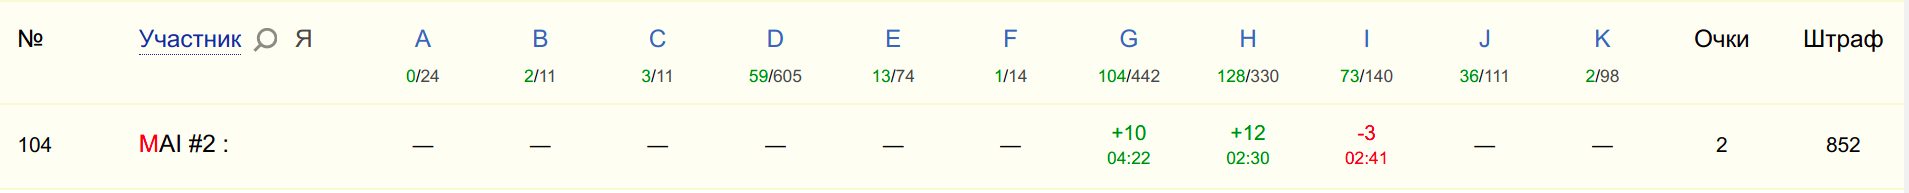
\includegraphics[scale=0.25]{images/gp_dolgop.png}\newline\noindent

\end{document}
